\begin{ZhChapter}

\chapter{Related Work}

\section{Metaheuristic}

\subsection{Evolving Algorithm}

\subsection{Genetic Algorithm}

\subsection{Genetic Programming}
In \cite{akhmedova2024generationlossfunctionimage}, a genetic programming-based method was proposed to find a better function for the image classification training task. They encoded the loss functions into trees, with each tree considered an individual. All individuals were aggregated into a population. In this study, the population was evolved across multiple generations. Before the start of each generation, all individuals were evaluated. Each individual had a probability of undergoing crossover with an individual from a special external archive to create a new individual; otherwise, it would perform the crossover with another individual. Following this, two probabilistic decisions were made. If successful, the new individual could perform subtree mutation or one-point mutation, respectively. At the end of each generation, the fitness value of all individuals was re-evaluated. A certain number of low-scoring individuals were eliminated to the special external archive mentioned earlier, maintaining the stability of the population's size. After these steps, a new generation began, continuing until a predefined number of generations was reached.By employing this method, this study successfully evolved an outstanding individual within the population, creating a function that could train an image classification model more effectively compared to Cross Entropy.

\section{Loss Function}

\subsection{Deep Learning Model}

\subsection{Importance of Loss Function}
In \cite{gonzalez2020improvedtrainingspeedaccuracy}, a loss function meet genetic programming is proposed ....
\section{Image Classification}

% \subsection{}
% 定義定義定義定義定義定義\cite{latex2e},定義定義定義定義,定義定義定義定義定義定義定義定義定義定義,定義定義。

% \begin{table*}[htbp]
%     \centering
%     \caption{表格範例標題} \label{tab: complexity}
%     \makebox[\linewidth][c]{
%     \renewcommand\arraystretch{1.2}{
%         \begin{tabular}{| l | c  c  c  c |}
%         \hline
%         Protocol & $P$ & $CS_1$ & $CS_2$ & $RG$ \\
%         \hline
%         MSSMul & $O(1)$, $O(1)$, N/A & $O(n-t)$, $O(n)$, $O(1)$ & $O(n-t)$, $O(n)$, N/A & $O(1)$, $O(n)$, $O(n)$ \\
%         SC & $O(1)$, $O(1)$, N/A & $O(n-t)$, $O(n)$, $O(1)$ & $O(n-t)$, $O(n)$, N/A & $O(1)$, $O(n)$, $O(n)$ \\
%         \hline 
%         \end {tabular}
%     }}
% \end {table*}

% \section{模型說明(小標)}

% 說明說明說明說明,說明說明說明說明說明說明說明說明說明說明說明說明,說明說明說明說明說明說明說明說明。

% \begin{figure*}[htbp]
%     \centering
%     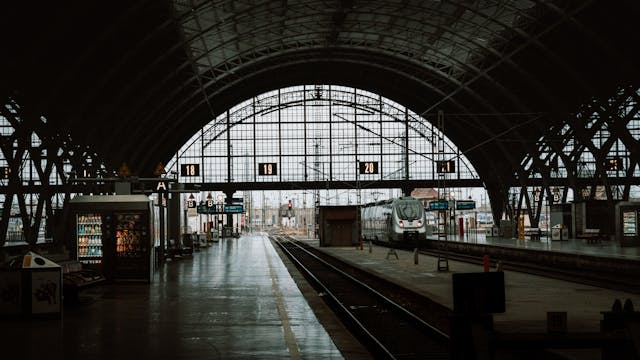
\includegraphics[width = 0.5\textwidth]{image.jpeg}
%     \caption{Cool train station}
%     \label{fig: image}
% \end{figure*}

\end{ZhChapter}